% *** LaTeX-mal for labrapporter i fysikk, v.14.08.2017 ***

% Dette er et eksempel på et LaTeX-dokument, og du kan bruke dette som et utgangspunkt for din egen rapport. Merk at for å kunne kompilere dokumentet uten feil, må du også laste ned filen pendel-oppdatert.pdf.
%
% Her i starten og videre nedover i teksten under har vi lagt inn en god del linjer som starter med tegnet "%". Disse linjene er kommentarer og synes ikke i det ferdige dokumentet. Vi kan også sette inn et kommentartegn midt på en linje. Alt som kommer før tegnet brukes da i kompileringen, mens resten av linja er en kommentar. 
%
% Kildefilen (.tex-filen) begynner alltid med et "preabmle". Her setter man opp innstillingene som brukes av kompilatoren til å utforme det ferdige dokumentet. Selve dokumentet begynner ikke før vi skriver \begin{document}.
%
% Dokumentasjon for alle pakker finnes på CTAN (http://www.ctan.org/)

%%%%%%%%%%%%%%%%%%%%%%%%%%%%%%%%%%%%%
% Preamble
%%%%%%%%%%%%%%%%%%%%%%%%%%%%%%%%%%%%%

\documentclass[5p,sort&compress]{elsarticle}		
% 5p gir 2 kolonner pr side. 1p gir 1 kolonne pr side.
% Valget sort&compress gjør at referansen [1,2,3] settes som [1-3]. 
% Andre innstillinger for "klassen" elsarticle finnes i dokumentasjonen på CTAN (http://www.ctan.org/pkg/elsarticle)

% Klassen elsarticle er laget for bruk i engelskspråklige tiksskrift. I blokken under bruker vi litt lavnivå TeX-magi for å redefinere bunnteksten på tittelsiden. Ikke bekymre deg for denne biten med kode, det som kommer lengere nede i dokumentet er lettere å forstå!
\makeatletter
\def\ps@pprintTitle{%
 \let\@oddhead\@empty
 \let\@evenhead\@empty
 \def\@oddfoot{\footnotesize\itshape
       Utkast levert til Veileder	% Bytt ut "Veileder" med navnet på veilederen din!
       \hfill\today}%
 \let\@evenfoot\@oddfoot}
\makeatother

% Encoding for input i tex-filen og encoding for output i pdf-filen
\usepackage[utf8]{inputenc}
\usepackage[T1]{fontenc}
\usepackage{textcomp}

% Last inn en font-pakke. Her bruker vi standard-fonten til LaTeX. 
\usepackage{lmodern}

% LaTeX gjør mye av typografien for deg, blant annet orddeling ved linjeskift og automatisk utfylling av endel tekst. For å kunne gjøre dette må kompilatoren vite hvilket språk dokumentet er skrevet på. 
\usepackage[norsk]{babel}
\usepackage[fixlanguage]{babelbib}
% Til tross for at vi har fortalt kompilatoren at vi skriver på norsk må vi fortelle den eksplisitt at vi ønsker at seksjonen "abstract" skal kalles "sammendrag"
\renewenvironment{abstract}{\global\setbox\absbox=\vbox\bgroup
\hsize=\textwidth\def\baselinestretch{1}%
\noindent\unskip\textbf{Sammendrag}
\par\medskip\noindent\unskip\ignorespaces}
{\egroup}

% Mikrotypografiske optimeringer
\usepackage[babel=true]{microtype}

% AMS-utvidelsene for å håndtere matematikk
\usepackage{amsmath}
\usepackage{amssymb}
\usepackage{bm}

% Måltall og enheter er spesielle typografiske dyr som reguleres av strenge regler. For å gjøre det enklere å håndtere tall og enheter på riktig måte bruker vi pakken siunitx.
\usepackage{siunitx}
% Vi tilpasser standardinstillingene til pakken til norske regler. 
\sisetup{
exponent-product = \cdot,
output-decimal-marker  =  {,}, % Pass på å endre desimalskilletegnet til punktum om du skriver på engelsk!
separate-uncertainty = true,
per-mode = symbol,
group-digits = false,
}

% Figurer og tabeller
\usepackage{graphicx} % Denne pakken er standard for å kunne laste inn figurfiler med ulike formater
% Løsne opp på de alt for strenge standardinstillingene for plassering av figurer og tabeller (floats) i LaTeX-kjernen
\renewcommand{\topfraction}{.85}
\renewcommand{\bottomfraction}{.7}
\renewcommand{\textfraction}{.15}
\renewcommand{\floatpagefraction}{.66}
\setcounter{topnumber}{3}
\setcounter{bottomnumber}{2}
\setcounter{totalnumber}{10}
\usepackage{flafter} % For å plassere floats i PDFen første sted LaTeX tillater etter det punktet de er definert i TeX-filen. Om du definerer figuren i TeX-filen rett etter at du refererer til den for første gang vil denne pakken sørge for at de fleste floats havner på greie steder
\usepackage{booktabs} % Denne pakken gir tilgang på endel ekstra kommandoer som legger til rette for god skikk og bruk i tabellformatering.
\usepackage{multirow}
\usepackage[font=small,labelfont=bf]{caption}	% Justering av LaTeX standarder for figurtekst og tabelltekst.

% Hyperreferanser
\usepackage[colorlinks=true,allcolors=blue]{hyperref}
% Noen av navnene for autoreferanser mangler på norsk, så vi ordner opp i det.
\addto\extrasnorsk{%
\def\figureautorefname{figur}%
\def\tableautorefname{tabell}%
\def\sectionautorefname{avsnitt}%
\def\subsectionautorefname{underavsnitt}%
\def\equationautorefname~#1\null{ligning~(#1)\null}
}
% Vi endrer fonten som brukes for URLer til den vanlige tekstfonten.
\urlstyle{same}

%%%%%%%%%%%%%%%%%%%%%%%%%%%%%%%%%%%%%
% Selve dokumentet
%%%%%%%%%%%%%%%%%%%%%%%%%%%%%%%%%%%%%

\begin{document}

% I "front matter" angir vi formalia knyttet til dokumentet -- tittel, forfatter, tilknytning og sammendrag
\begin{frontmatter}

\title{Mal for rapport til laboratorium i fysikk}

% I forfatterlisten legger vi inn "ikke-brytende" mellomrom etter initialene
\author{J.~O.~Bruun}
\author{S.~Klyve}

\begin{abstract}
Sammendraget er en kort og konsis oppsummering av innholdet i rapporten. Sammendraget er den delen av rapporten som skal skrives sist, når du har full kontroll på alt innholdet. En god lengde for et sammendrag er 4--5 setninger. I løpet av disse setningene skal forsøket introduseres, du skal fortelle hvilke metoder som ble brukt, resultatene skal presenteres og du må fortelle kort hva resultatene betyr. Om resultatet eksisterer i form av et tallsvar skal dette oppgis med tilhørende usikkerhet. 
\end{abstract}

\end{frontmatter}


\section{Introduksjon}
Stefan-Boltzmanns lov er en viktig relasjon i fysikken, som forbinder emittert varmeenergi  fra et svart legeme, med dets temperatur. Den ble først formulert av Joseph Stefan i 1879, og utledet av Ludwig Boltzmann fem år senere (INSERT KILDE). I dette forsøket skal vi studere emissiviteten til ulike overflater ved ulike temperaturer, i tillegg til å verifisere Stefan-Boltzmanns lov ved å sjekke forholdet mellom temperatur og emittert varme fra et objekt.


Her begynner den egentlige rapporten. Mer informasjon om hva de enkelte delene av rapporten skal inneholde finnes på nettsiden til laben~\cite{labside}. På slutten av forrige setning ser vi et eksempel på en referanse. Her er et eksempel på en referanse til læreboka~\cite{Young2016}. Referanselisten kommer til slutt i rapporten. I denne malen har vi brukt \textsc{Bib}\TeX\ til å formatere referansene, men det er også mulig å formatere dem manuelt direkte i \texttt{tex}-filen. 
% BibTeX er det programmet som tradisjonelt brukes til automatisert referansehåndtering i LaTeX. Den mest moderne måten å håndtere referanser på er pakken biblatex, men den kan ikke brukes sammen med elsarticle.



\section{Teori}
Et svart legeme er et objekt som absorberer all innkommende strålingsenergi, uavhengig av bølgelengden. Dersom objektet er i termisk likevekt, blir det totalt sett hverken tilført eller avgitt energi. Det vil si at objektet må emittere like mye stråling som det absorberer for å oppnå likevekt. For et svart legeme betyr dette at den emitterte strålingsenergien er lik den absorberte. Forholdet mellom den emitterte effekten per flateenhet, $j$, og det svarte legemets temperatur er gitt ved Stefan-Boltzmanns lov:

\begin{equation}
  j = \sigma T^4
\label{eq:SB} % Merkelappen til ligningen er det navnet vi bruker når vi skal referere til ligningen senere.
\end{equation}

Her er $\sigma = \SI{5,67e-8}{\watt\metre^{-2}\kelvin^{-4}}$ Stefan-Boltzmann-konstanten. Dersom dette skal gjelde for et objekt med vilkårlig emissivitet $\epsilon$, må vi justere til

\begin{equation}
  j = \epsilon\sigma T^4.
\label{eq:SBepsilon} % Merkelappen til ligningen er det navnet vi bruker når vi skal referere til ligningen senere.
\end{equation}

Leslies kube er et objekt med fire ulike overflater; svart, hvit, upolert aluminium og blankt aluminium (speil). Den varmes opp innvendig ved hjelp av en glødepære, og temperaturen til kuben kan leses av i tabell basert på resistansen i en innebygd termistor. Når resistansen stabiliserer seg på en gitt verdi, har kuben oppnådd termostatisk likevekt. Fra dette kan det måles avgitt varmestråling med en strålingssensor, og med det undersøke hvordan dette avhenger med overflate og temperatur.

For å måle temperaturen til glødetråden i en Stefan-Boltzmann-lampe, kan følgende relasjon brukes:

\begin{equation}
  T=T_0+\frac{R-R_0}{\alpha R_0}
\label{eq:TempMetall} 
\end{equation}

Her er $\alpha=\SI{4,5e-3}{\kelvin^{-1}}$ temperaturkoeffisienten til wolfram. $R_0$ er motstanden ved referansetemperatur $T_0$, og $R=\frac{V}{I}$ er motstand ved temperatur $T$. Siden denne relasjonen i utgangspunktet gjelder kun for små temperaturvariasjoner i metallet, må vi bruke relativ motstand $R/R_0$, og lese av temperaturen til wolframtråden fra tabell. Fra dette finner vi usikkerheten i den relative resistansen ved Gauss feilforplantning

\begin{equation}
  \label{eq:ErrorRelRes}
  \left( \Delta \frac{R}{R_{0}} \right) ^{2} = \frac{\Delta R^{2}}{R_{0}^{2}} + \frac{R^{2} \Delta R_{0}^{2}}{R_{0}^{4}}.
\end{equation}


\begin{figure}
  \centering
  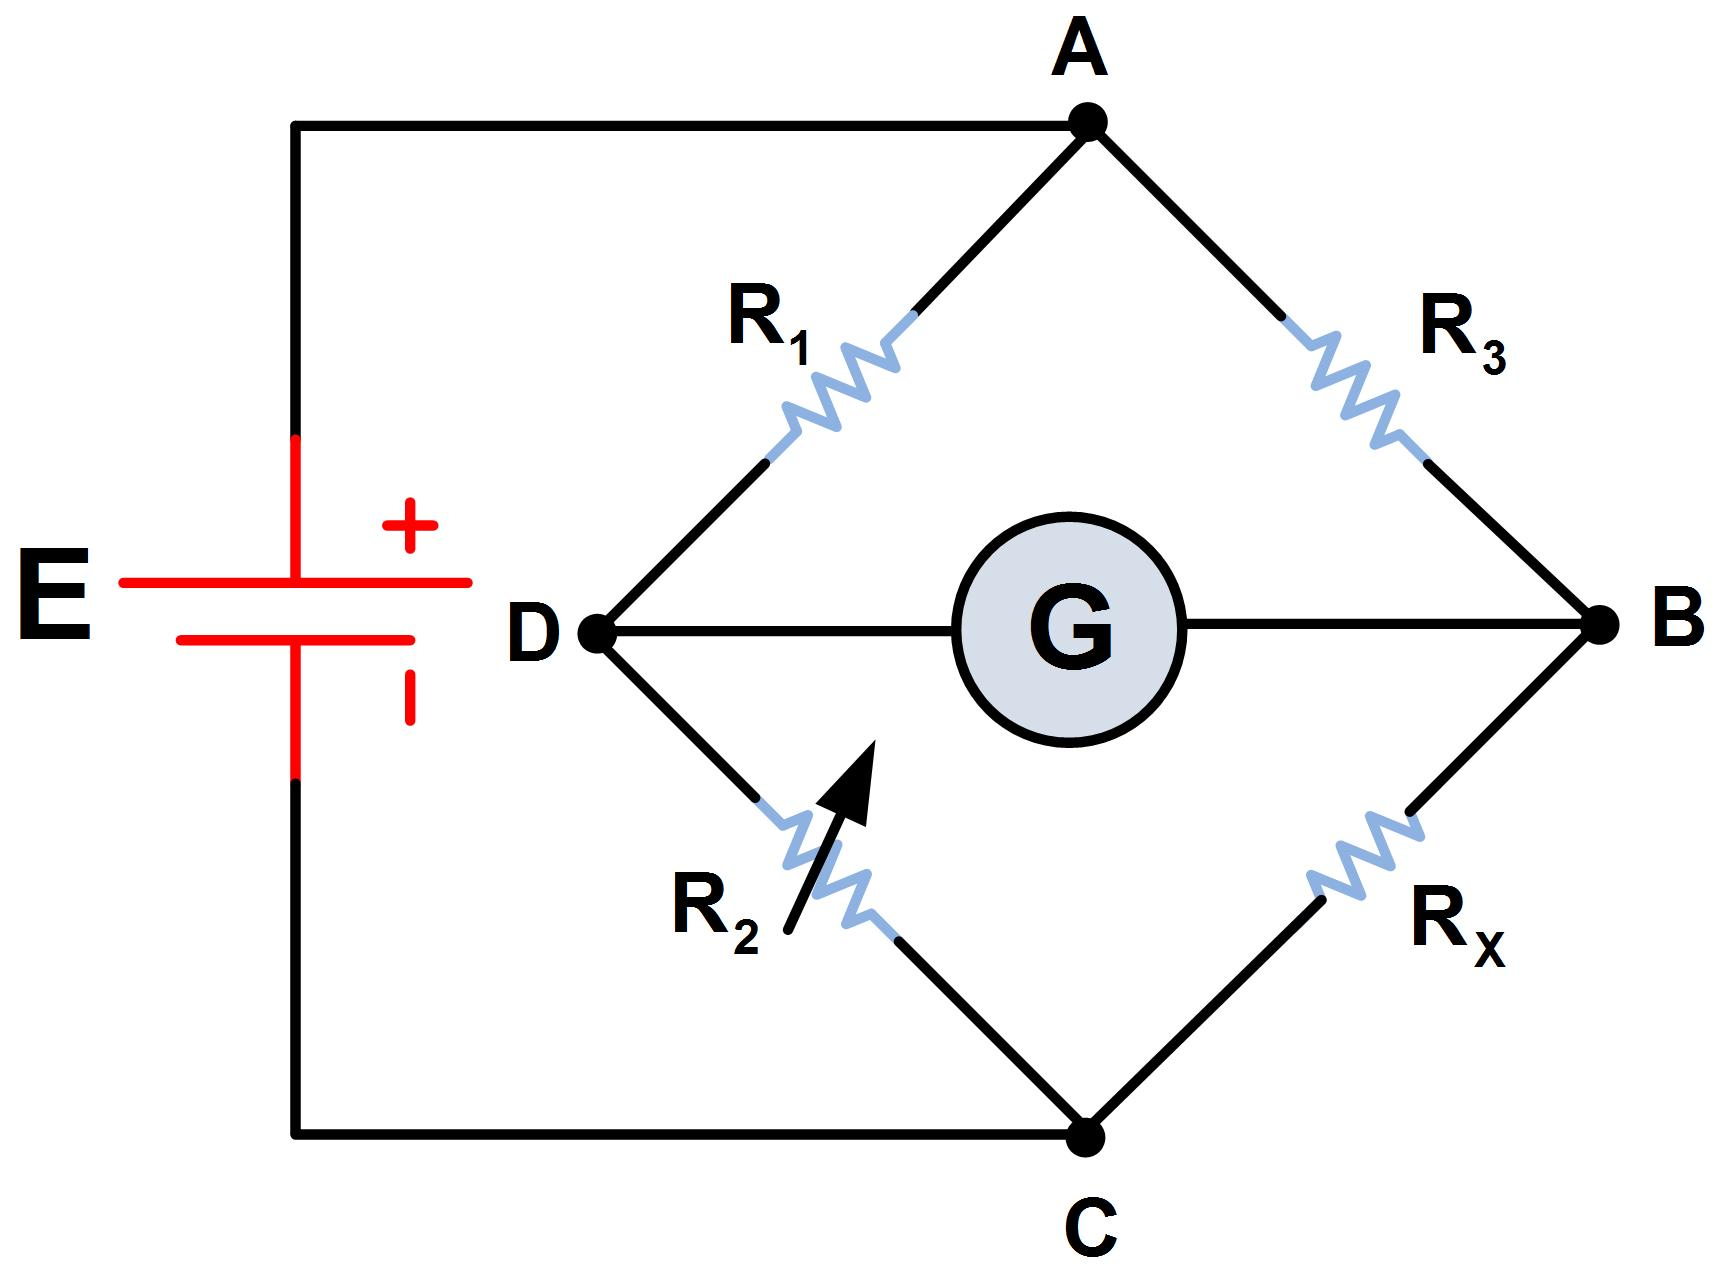
\includegraphics[width=0.30\textwidth]{wheat.jpg}
  \caption{Wheatstonebro \cite{wheatstone}. $R_{1}, R_{2}, R_{3}$ er kjente størrelser som kan justeres helt til det ikke går strøm gjennom $G$.}
  \label{fig:Wheatstone}
\end{figure}

En Wheatstonebro kan brukes til å måle nøyaktig motstand i en krets. Ved å justere resistansene vist i \autoref{fig:Wheatstone} til strømmen gjennom $G$ er 0, så kan en ved Krichoffs lover finne resistansen
\begin{equation}
  \label{eq:Wheatstone}
  R_{x} = \frac{R_{3} R_{2}}{R_{1}}.
\end{equation}
Siden $R_{x}$ her vil referere til resistansen i resistoren i tillegg til i ledningene kan en finne resistansen i resistoren $R_{0}$ ved å kople den ut og finne resistansen i ledningene $R_{x0}$ og har dermed
\begin{equation}
  \label{eq:WheatstoneReal}
  R_{0} = R_{x} - R_{x0}.
\end{equation}
Feilmarginen i $R_{0}$ kan da finnes ved Gauss feilforplantning
\begin{align}
  \label{eq:ErrorBridge}
  \Delta R_{0}^{2} =& \frac{(R_{x} - R_{x0})^{2}}{R_{1}^{2}} \left( \Delta R_{3}^{2} + \frac{R_{3}^{2} \Delta R_{1}^{2}}{R_{1}^{2}} \right) \notag \\
  &+ \frac{R_{3}^{2}}{R_{1}^{2}} \left( \Delta R_{x}^{2} + \Delta R_{x0}^{2} \right).
\end{align}



\section{Metode}
Dette forsøket omfatter i hovedsak to ulike deler; først å undersøke emissivitet til ulike overflater ved ulike temperaturer ved bruk av en Leslies kube, og deretter verifisere Stefan-Boltzmann lov ved å måle emittert varmestråling fra en lampe ved varme temperaturer.


\begin{figure}
  \centering
  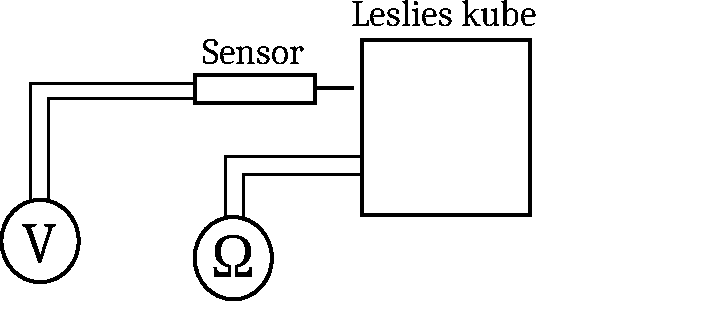
\includegraphics[width=0.4\textwidth]{figures/leslikube.pdf}
  \caption{Utstyrsoppsett. Leslies kube er koblet til et strømuttak og et ohmmeter, varmestrålingssensoren er koblet til et voltemeter.}
  \label{fig:Leslikube}
\end{figure}

For Leslies kube kobles utstyret opp som vist i \autoref{fig:Leslikube} og skrur på lampen i Leslies kuben på høy intesitet først før den skrus ned når ohmmeteteret viser omtrent $\SI{40}{\kilo\ohm}$ før intensiteten skrus ned. Venter så til det oppnås en form for termisk likevekt og måler så varmestråling ved å lese av voltmeteret koblet til sensoren på hver av de fire sidene og skrur så opp intensiteten, venter i omtrent fem minutter til det er tilnærmet termisk likevekt og måler så varmestråling på nytt. Gjør dette fire ganger.

\begin{figure}
  \centering
  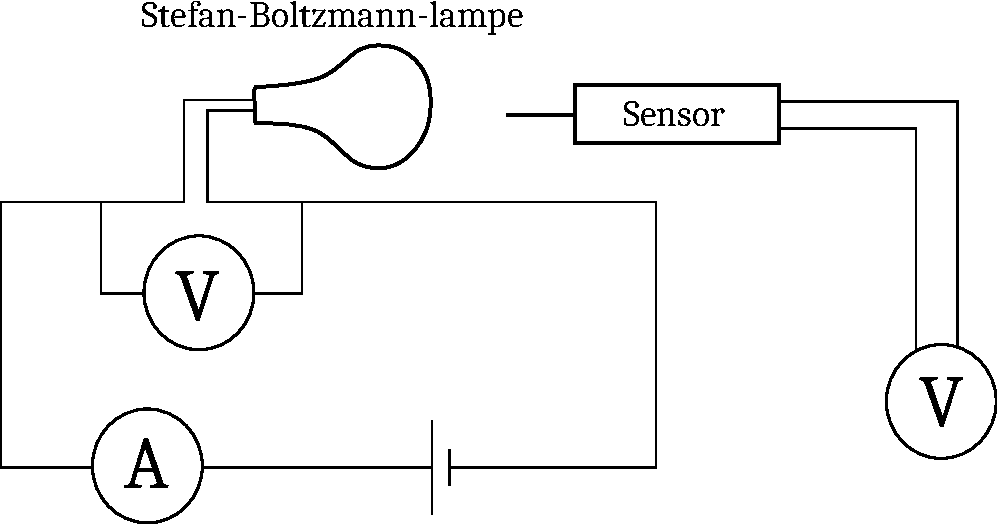
\includegraphics[width=0.4\textwidth]{figures/lampe.pdf}
  \caption{Utstyrsoppsett. Kobler et voltmeter paralelt med Stefan-Boltzmann-lampen i en krets med et ammeter og en spenningskilde som kobles til et strømuttak. Kobler et voltmeter til sensoren.}
  \label{fig:SBlampe}
\end{figure}

Kobler opp utstyr som vist i \autoref{fig:SBlampe}. Setter spenningen til $\SI{1}{\volt}$ og måler så av strøm og spenning i kretsen med Stefan-Boltzmann-lampen og spenningen i varmestrålingssensoren. Setter så opp spenningen med $\SI{1}{\volt}$ og gjør det samme til og med $\SI{12}{\volt}$.


\section{Resultater}
Ser først på dataen funnet ved Leslies kube som vist i \autoref{fig:LeslieResults}. Avlesninger av voltmeteret koblet til varmestrålingssensoren viser intensiteten og ved avlesninger av ohmmeteret finnes resistans og dermed temperatur ved avlesning av tabell. Siden temperaturen finnes ved avlesning av tabell finnes nederste og øverste grense ved avlesning av laveste resistans som kan slås opp høyere enn høyeste verdi i feilmarginintervallet, og motsatt for lavere.

\begin{figure}
  \centering
  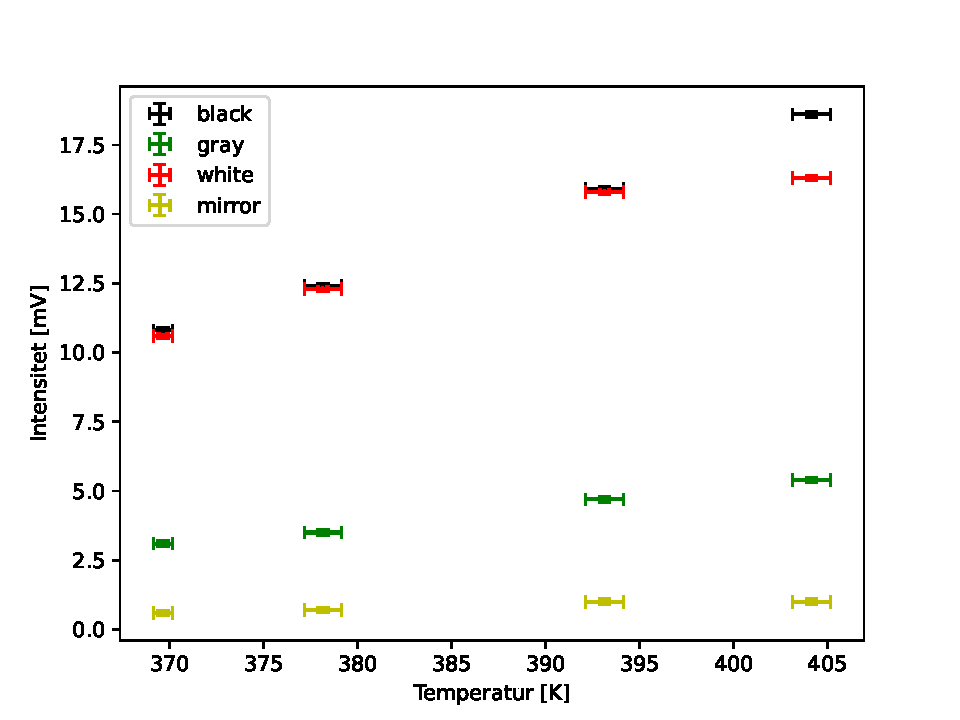
\includegraphics[width=0.4\textwidth]{../code/LC.pdf}
  \caption{Leslies kube. Punktene er målinger ved de forskjellige intensitetene hvor tempereaturen er tilnærmet konstant i hver av de fire målingene ved samme intensitetsinstilling.}
  \label{fig:LeslieResults}
\end{figure}

Videre er dataen for Stefan-Boltzmann-lampa vist i \autoref{fig:SBlampResults}. Ved avlesninger av voltmeteret koblet til sensoren finnes intensiteten og temperatur er funnet ved avlesning av resistans og ved å lese av tabell. Usikkerheten i temperaturen kommer av måleusikkerheten i resistansen og usikkerheten i resistansen ved romtemperatur som vist i \eqref{eq:ErrorRelRes}. Bruker samme metode for å finne feilmarginer som ved Leslies kube.

\begin{figure}
  \centering
  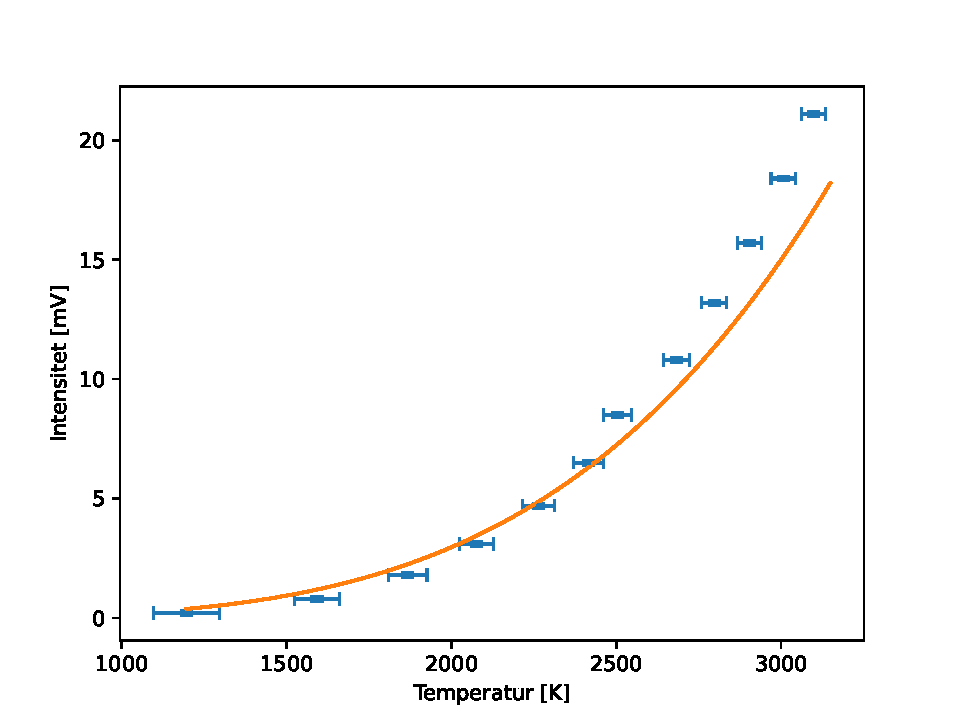
\includegraphics[width=0.4\textwidth]{../code/SB_lamp.pdf}
  \caption{Stefan-Boltzmann-lampe. Punktene er avlesninger og den heltrukkne linja er et gjett på en fjerdegradsfunksjon.}
  \label{fig:SBlampResults}
\end{figure}


\section{Diskusjon}
Kan se i \autoref{fig:LeslieResults} at alle målingene ser ut til å følge en lik økning å fothold til hverandre med unntak av den hvite siden i siste måling. Vi forventet at intensiteten skulle følge likningen i \eqref{eq:SBepsilon} med varierende $\epsilon$ på de forskjellige sidene. Da ville målingene vært proporsjonale med $T^{4}$, men hvis vi tegner inn $\alpha T^{4}$ med $\alpha=\overline{U} / T^{4}$, hvor $\overline{U}$ er gjennomsnittet av de målte verdiene for intensiteten, får vi grafen vist i \autoref{fig:LeslieResFunc}. Her er det vanskelig å se om denne modellen passer siden det er relativt liten forskjell på største og minste verdi for temperaturene som er målt.

\begin{figure}
  \centering
  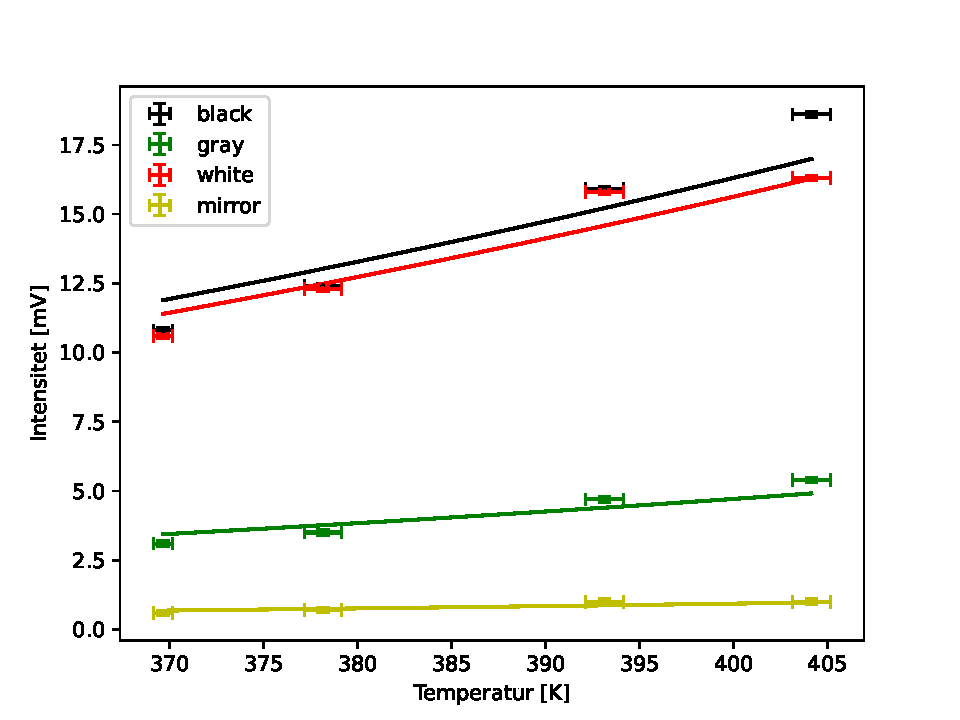
\includegraphics[width=0.4\textwidth]{../code/LC_graphs.pdf}
  \caption{Leslies kube med tilnærmede fjerdegradspolynomer.}
  \label{fig:LeslieResFunc}
\end{figure}

Det kan finnes flere forklaringer på hvorfor de teoretiske modellene som vi forventet ikke skulle vises i dataen. Noe som kan hende er at siden vi måler temperaturen ved resistans i en glødepære inne i kuben vil temperaturen vi finner være for glødepæren, men muligens ikke for overflaten på kuben og da kan det hende at systemet inne i kuben ikke er kommet i termisk likevekt å at temperaturen dermed ikke realistisk er det samme som den vi måler. Det kan hende at denne temperaturforskjellen øker med temperaturen vi måler og at målingene derfor ikke er proporsjonal med $T^{4}$.

Vi kan også tenke oss at siden denne temperaturen er så liten i forhold til romtemperaturen kan det gjøre at varmestrålingen er liten i forhold til annen stråling som kan detekteres av sensoren og dermed ikke vil øke med $T^{4}$, men i dette tilfellet er hovedsaklig problemet at temperaturforskjellene er liten og det er dermed vanskelig å konkludere med noen proporsjonalitet.

Vi kan så se på målingene i forhold til hverandre. Vi hadde regnet med at den svarte siden ville emittere mest stråling siden denne siden også vil absorbere mest stråling. Det som var uventet var at den hvite siden emitterte neste like mye som den svarte siden, ettersom vi vet at hvite objekter reflekterer alt synlig lys. Vi kan tenke oss at selv om dette er sant så vil i dette tilfelle varmestrålingen ikke være i form av synlig lys og det kan hende at den hvite siden absorberer denne bølgelengden nesten like godt som den svarte siden og dermed emitterer omtrent like mye.

Vi ser at det er en måling som er langt ganske langt unna den korresponderende målingen av den svarte siden. Dette kan være en målefeil, men kan tenke seg at i dette tilfellet begynner varmestrålingen å nærme seg synlig lys eller en annen bølgelengde som blir reflektert av hvitt og ikke svart. Dette virker ikke veldig sannsynlig siden vi vet at intensiteten i varmestrålingen skal øke med $T^{4}$ og det derfor ikke gir mening at det er en stor plutselig forskjell i evnen til absorpsjon. En annen tanke er at det egentlig er en betydelig forskjell på disse målingene men at de ser små ut i forhold til alle de andre målingene vi har. Det kan også hende at det tar lenger å tid å varme opp visse sider av kuben og at dette fører til at hvit emitterer omtrent like mye stråling. Dette siste punktet er nok ikke spesielt sannsynlig siden vi til første måling lot det stå veldig lenge og vi ser at første måling også er veldig like.

\begin{table}
  \centering
  \caption{Emisjonskonstant for de ulike overflatene på Leslies kube.}
  \begin{tabular}{cc}
    \toprule
    Side & $\epsilon$ \\
    \midrule
    Svart & $\SI{1}{}$ \\
    Hvit & $\SI{0.94(7)}{}$ \\
    Upolert aluminium & $\SI{0.29(2)}{}$ \\
    Polert aluminium & $\SI{0.06(2)}{}$ \\
    \bottomrule
  \end{tabular}
  \label{tab:LeslieEmisjonsevne}
\end{table}

Som forventet er den blanke aluminiumssiden som emitterer minst da dette omtrent er et speil og vil dermed reflektere omtrent all stråling. I tillegg vet vi at aluminium reflekterer mye stråling fra før av, noe vi også kan se ved at den upolerte aluminiumssiden også emitterer ganske lite, men likevel en del mere enn den blankpolerte. For å finne emisjonskonstanter for upolert og blankpolert aluminium kan det antas at den svarte siden er tilnærmet et svart legeme og vil dermed ha $\epsilon = 1$ og får da \autoref{tab:LeslieEmisjonsevne}. Her er det regnet ut $\epsilon = j/j_{b}$ hvor $j_{b}$ er strålingen fra den svarte siden da vi antar dette er et svart legeme. Feilmarginen er funnet ved Gauss feilforplantning og så finne ekstremalverdiene med feilmarginer for de ulike målingene.

\begin{figure}
  \centering
  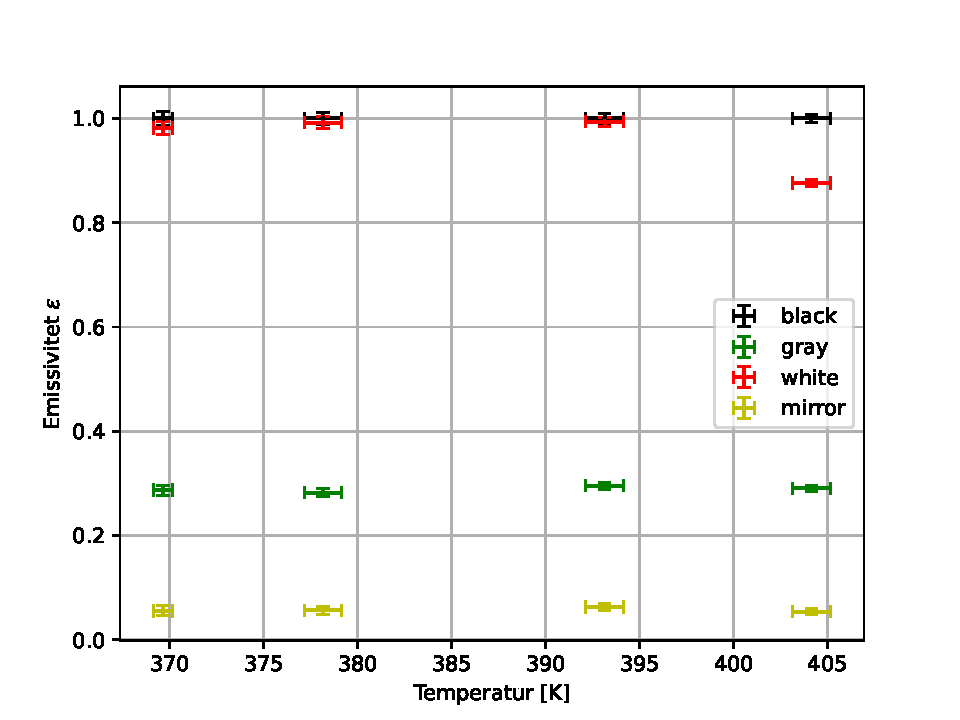
\includegraphics[width=0.4\textwidth]{../code/LC_emissivity.pdf}
  \caption{Emissivitet på Leslies kube ved svart side antatt et perfekt svart legeme.}
  \label{fig:LesliesEmissivity}
\end{figure}

Kan også ved å se på \autoref{fig:LesliesEmissivity} at emissiviteten ser uavhengig ut fra temperaturen, med unntak fra siste måling på hvit side, noe vi ville forventet fra teorien. Igjen ser en at den hvite siden opptrer veldig likt som et svart legeme, noe som ikke virker intuitivt. Ser også at dermed en ser bort ifra siste måling på hvit side får en $\epsilon = \SI{0.99(2)}{}$. Dette er overraskende nærme et svart legeme, men har også en feilmargin som gir en mulig verdi $\epsilon > 1$, noe som ikke er mulig. Siden det er antatt at den svarte siden kan ses på som et perfekt svart legeme, noe som ikke er riktig, så gir det mulig mening at dette kan skje. Her kan det muligens også ha noe å si at de forskjellige sidene på kuben varmes opp på ulik tid og dermed kan temperaturen være forskjellige på de forskjellige sidene.

\section{Konklusjon}
Nå har vi gitt endel eksempler på formatering. For å mestre \LaTeX\ er det bare én ting som gjelder -- trening. Last ned kildefilene og lek med de ulike elementene. Sitter du fast er det som regel noen som har hatt de samme problemene før deg. Det meste av dokumentasjon er å finne på \href{http://www.ctan.org/}{CTAN}. Spørsmål og svar er å finne på \href{http://tex.stackexchange.com/}{\LaTeX\ StackExchange}. Lykke til!

% Her kommer referanselisten
\begingroup
\begin{center}
\rule{2cm}{.4pt} % Vi markerer starten på referanselisten med en horisontal strek
\end{center}
\makeatletter
\@beginparpenalty=10000 % Vi setter en høy straff for kompilatoren om den setter inn et sideskift mellom streken og starten på referanselisten.
\makeatother
\bibliographystyle{babunsrt}
\bibliography{referanseliste}
\endgroup

\end{document}
